\documentclass{article}
\usepackage[utf8]{inputenc}
\usepackage{amsmath}
\usepackage{amssymb}
\usepackage{graphicx}
\usepackage{hyperref}
\usepackage{tikz}
\usepackage{pgfplots}
\usepackage{float}
\usepackage{listings}
\usepackage{color}
\usepackage{bbm}
\usepackage{multirow}

\title{Reinforcement Learning \\ Exercise 5 - Solution}
\author{Jonathan Schnitzler - st166934 \\
Eric Choquet - st160996}
\date{\today}
\begin{document}
\maketitle
\section*{Task 1) - Random Walk}
In the Random walk example from lecture 5 slide 12 the value is a prediction of the probability of terminating on the right side of the chain. Let us first recall the update rule for $TD(0)$:
\begin{equation}
    V(S_t) \leftarrow V(S_t) + \alpha \left[ R_{t+1} + \gamma V(S_{t+1}) - V(S_t) \right]
\end{equation}
When only the first state $V(A)$ is updated, the sampled Random walk is immediately terminated at the left. Then the equation abouve evaluates to
\begin{equation}
    V(A) \leftarrow V(A) + 0.1 \left[ 0 + 0 - V(A) \right] = V(A) - 0.1 V(A) = 0.5 - 0.1 \cdot 0.5 = 0.45
\end{equation}
Otherwise, also the state of another value would have been changed, e.g. if first the Random walk would have gone to the right, then $V(B)$ would have been updated as well.

\section*{Task 2) - Sarsa and Q-learning on the Frozen Lake}

\paragraph*{a) - Sarsa}

The Sarsa algorithm is implemented in the accompanying python file. The algorithm is run for 10,000 episodes with a learning rate of $\alpha = 0.1$ and a discount factor of $\gamma = 0.9$. The results are shown in the following figures. One notices that the tiles with value 0 are either holes or the goal. The algorithm has learned to avoid the holes and reach the goal in the lower right corner.

\begin{figure}[H]
\centering
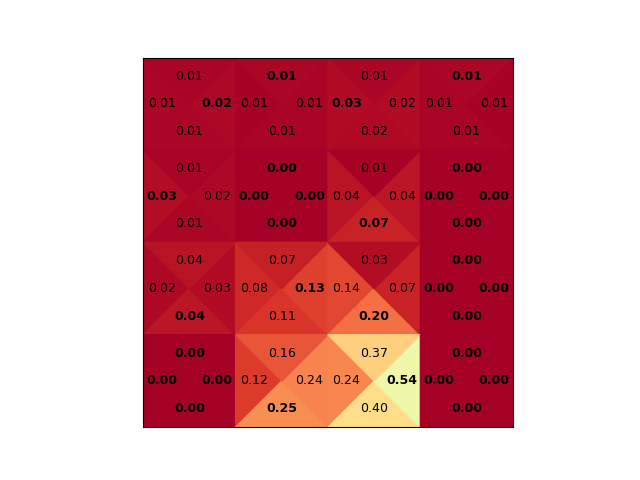
\includegraphics[width=0.9\textwidth]{figures/Q_sarsa_slippery.png}
\caption{Action-value matrix Q for Sarsa on the Frozen Lake}
\label{fig:Q_sarsa}
\end{figure}

\begin{figure}[H]
\centering
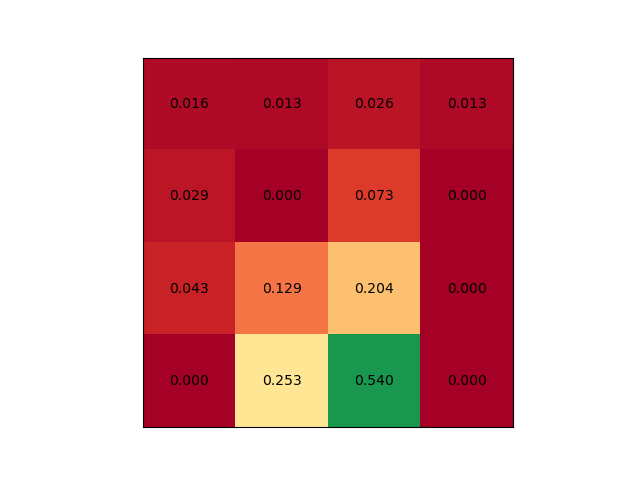
\includegraphics[width=0.9\textwidth]{figures/V_sarsa_slippery.png}
\caption{Value matrix V for sarsa on the Frozen Lake}
\label{fig:V_sarsa}
\end{figure}

\begin{figure}[H]
\centering
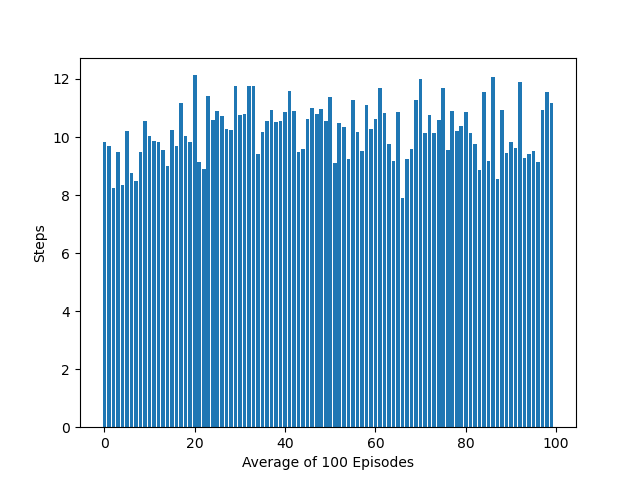
\includegraphics[width=0.9\textwidth]{figures/Avg_Episode_sarsa.png}
\caption{Average episode length as training continues}
\label{fig:avg_sarsa}
\end{figure}

\paragraph*{b) Q-learning}

The Q-learning algorithm is implemented in the accompanying python file. The algorithm is run for 10,000 episodes with a learning rate of $\alpha = 0.1$ and a discount factor of $\gamma = 0.9$. The results are shown in the following figures. The main difference is that for the update step the maximum over all possible actions is taken, instead of the action that is actually taken. Therefore the performance during training is worse, then the performance for optimal policy.

\begin{figure}[H]
\centering
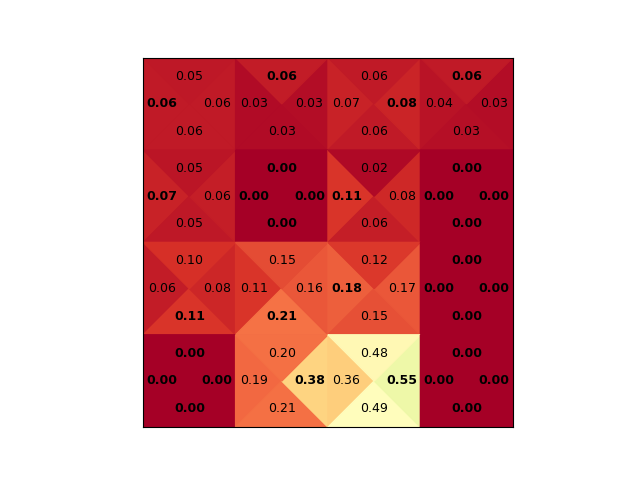
\includegraphics[width=0.9\textwidth]{figures/Q_q_slippery.png}
\caption{Action-value matrix Q for Q-learning on the Frozen Lake}
\label{fig:Q_q}
\end{figure}

\begin{figure}[H]
\centering
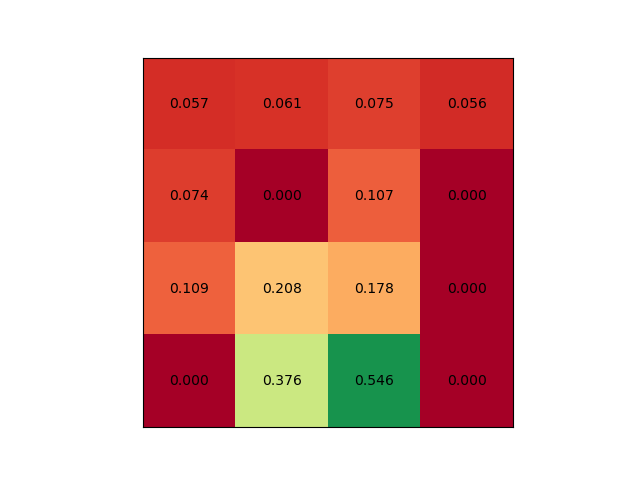
\includegraphics[width=0.9\textwidth]{figures/V_q_slippery.png}
\caption{Value matrix V for Q-learning on the Frozen Lake}
\label{fig:V_q}
\end{figure}



\paragraph*{c) Deterministic policy}

The same plots but now evaluated for the deterministic policy of the frozen lake. Q learning outperforms Sarsa in this case.

\begin{figure}[H]
\centering
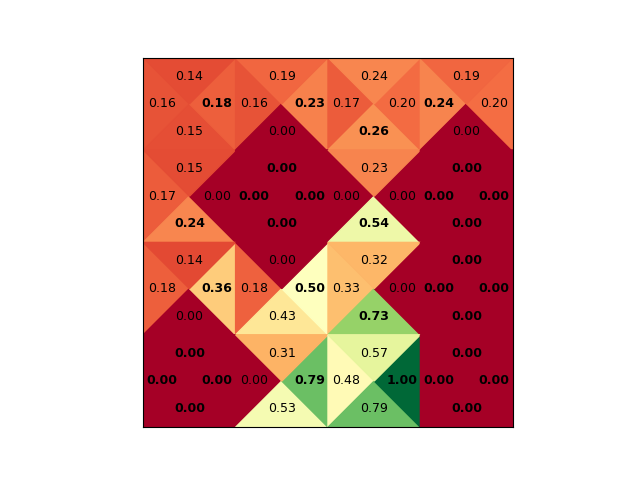
\includegraphics[width=0.9\textwidth]{figures/Q_sarsa_det.png}
\caption{Deterministic Action-value matrix Q for Sarsa on the Frozen Lake}
\label{fig:Q_sarsa_det}
\end{figure}

\begin{figure}[H]
\centering
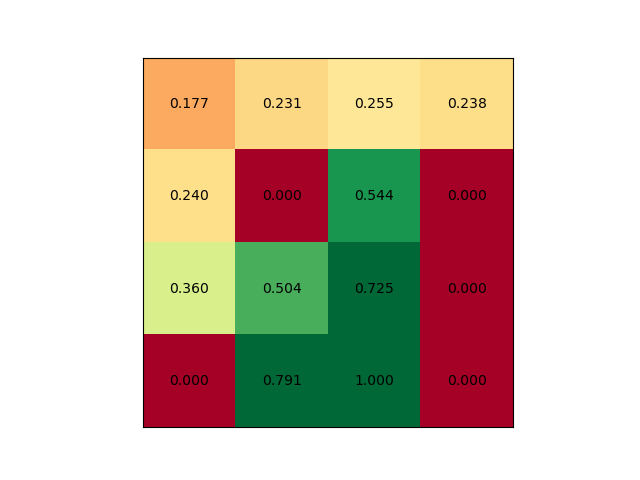
\includegraphics[width=0.9\textwidth]{figures/V_sarsa_det.png}
\caption{Deterministic Value matrix V for sarsa on the Frozen Lake}
\label{fig:V_sarsa_det}
\end{figure}



\begin{figure}[H]
\centering
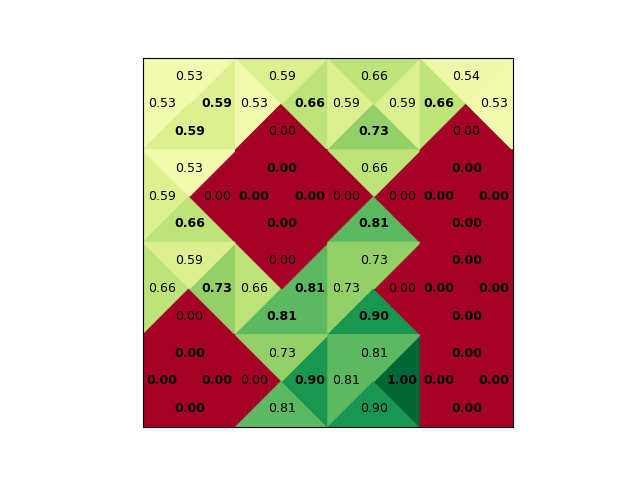
\includegraphics[width=0.9\textwidth]{figures/Q_q_det.png}
\caption{Deterministic Action-value matrix Q for Q-learning on the Frozen Lake}
\label{fig:Q_q_det}
\end{figure}

\begin{figure}[H]
\centering
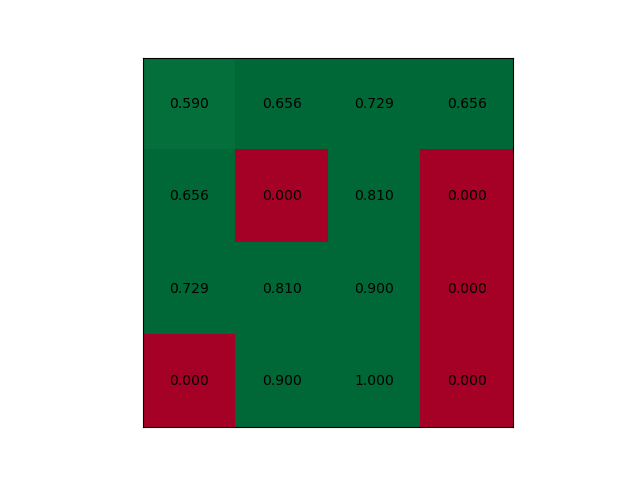
\includegraphics[width=0.9\textwidth]{figures/V_q_det.png}
\caption{Deterministic Value matrix V for Q-learning on the Frozen Lake}
\label{fig:V_q_det}
\end{figure}



\paragraph*{d) - Larger grid}

For the larger 8x8 grid 1,000,000 episodes were run for both algorithms, as otherwise the convergence was not reached. The results for sarsa are shown.

\begin{figure}[H]
\centering
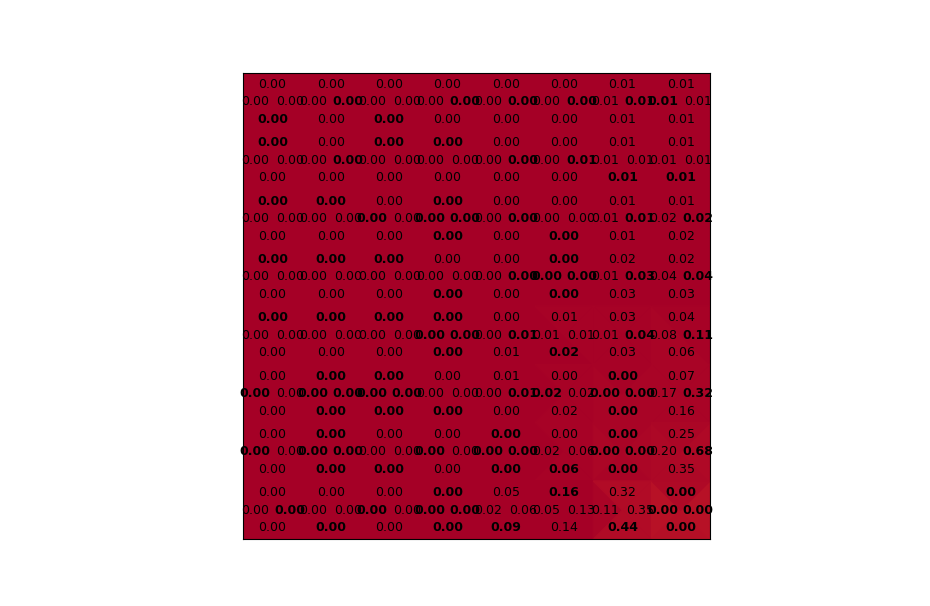
\includegraphics[width=0.9\textwidth]{figures/Long_Q_sarsa.png}
\caption{Action-value matrix Q for Sarsa on the Frozen Lake 8x8 grid}
\label{fig:long_q_sarsa}
\end{figure}

\begin{figure}[H]
\centering
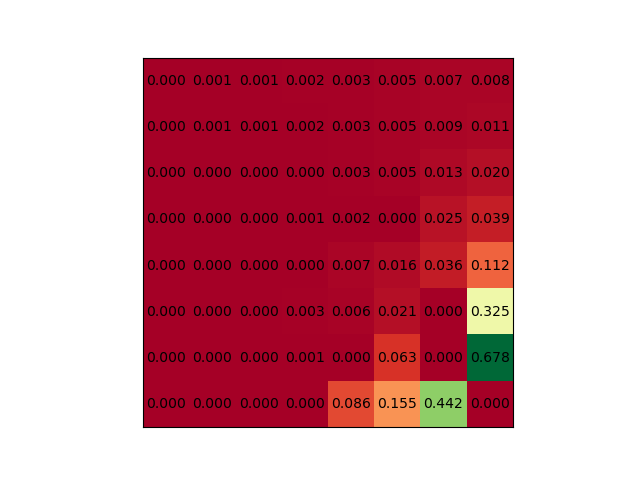
\includegraphics[width=0.9\textwidth]{figures/Long_V_sarsa.png}
\caption{Value matrix V for sarsa on the Frozen Lake 8x8 grid}
\label{fig:long_v_sarsa}
\end{figure}




\end{document}













